%
% teil1.tex -- Mathematischer Hintergrund
%
% (c) 2022 Fabian Dünki, Hochschule Rapperswil
%
\section{Mathematischer Hintergrund
\label{0f1:section:mathHintergrund}}
\rhead{Mathematischer Hintergrund}

\subsection{Hypergeometrische Funktion $\mathstrut_0F_1$
\label{0f1:subsection:0f1}}
Wie in Kapitel \ref{buch:rekursion:section:hypergeometrische-funktion} beschrieben,
wird die Funktion $\mathstrut_0F_1$ folgendermassen definiert.
\begin{definition}
    \label{0f1:rekursion:hypergeometrisch:def}
    Die hypergeometrische Funktion
    $\mathstrut_0F_1$ ist definiert durch die Reihe
    \[
    \mathstrut_0F_1
    \biggl(
    \begin{matrix}
    \\
    b_1
    \end{matrix}
    ;
    x
    \biggr)
    =
    \mathstrut_0F_1(;b_1;x)
    =
    \sum_{k=0}^\infty
    \frac{1}{(b_1)_k}\frac{x^k}{k!}.
    \]
\end{definition}


\subsection{Airy Funktion
\label{0f1:subsection:airy}}
Wie in \ref{buch:differentialgleichungen:section:hypergeometrisch} dargestellt, ist die Airy-Differentialgleichung
folgendermassen definiert.
\begin{definition}
    y'' - xy = 0
    \label{0f1:airy:eq:differentialgleichung}
\end{definition}

Daraus ergibt sich wie in Aufgabe~\ref{503} gefundenen Lösungen der
Airy-Differentialgleichung als hypergeometrische Funktionen.


\begin{align*}
y_1(x)
=
\sum_{k=0}^\infty
\frac{1}{(\frac23)_k} \frac{1}{k!}\biggl(\frac{x^3}{9}\biggr)^k
=
\mathstrut_0F_1\biggl(
\begin{matrix}\text{---}\\\frac23\end{matrix};\frac{x^3}{9}
\biggr).
\\
y_2(x)
=
\sum_{k=0}^\infty
\frac{1}{(\frac43)_k} \frac{1}{k!}\biggl(\frac{x^3}{9}\biggr)^k
=
x\cdot\mathstrut_0F_1\biggl(
\begin{matrix}\text{---}\\\frac43\end{matrix};
\frac{x^3}{9}
\biggr).
\qedhere
\end{align*}


\begin{figure}
    \centering
    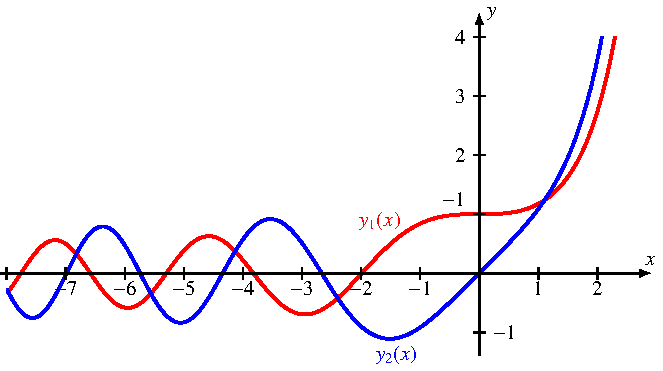
\includegraphics{papers/0f1/images/airy.pdf}
    \caption{Plot der Lösungen der Airy-Differentialgleichung $y''-xy=0$
    zu den Anfangsbedingungen $y(0)=1$ und $y'(0)=0$ in {\color{red}rot}
    und $y(0)=0$ und $y'(0)=1$ in {\color{blue}blau}.
    \label{0f1:airy:plot:vorgabe}}
\end{figure}